\documentclass[pdf, unicode, 12pt, a4paper,oneside,fleqn]{article}

\usepackage{styles/log-style}
\begin{document}

\begin{titlepage}
\begin{center}
\bfseries
{\Large Московский авиационный институт\\ (национальный исследовательский университет)}

\vspace{48pt}
{\large Факультет информационных технологий и прикладной математики}

\vspace{36pt}
{\large Кафедра вычислительной математики и программирования}

\vspace{48pt}Лабораторная работа \textnumero 2 по курсу 
\enquote{Численные методы}
\end{center}
\vspace{72pt}

\begin{flushright}
\begin{tabular}{rl}
Студент: & П.\,А. Гамов \\
Преподаватель: & Д.\,Л. Ревизников \\
Группа: & М8О-407Б \\
Дата: & \\
Оценка: & \\
Подпись: & \\
\end{tabular}
\end{flushright}
\vfill
\begin{center}
\bfseries
Москва, \the\year
\end{center}
\end{titlepage}

\pagebreak

\section{Решение нелинейных уравнений}

Данная функция.
\begin{lstlisting}
def f(x):
    return x**3 + x**2 - x - 0.5
\end{lstlisting}

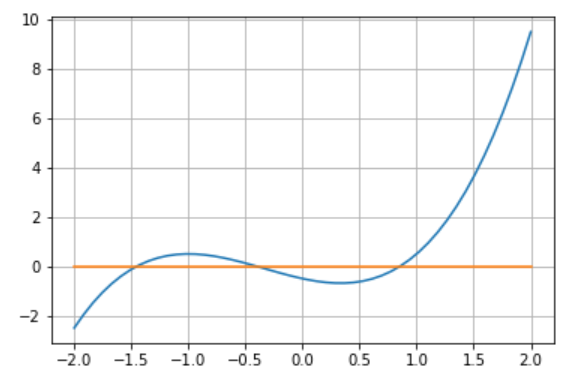
\includegraphics[scale=0.6]{data2lab.png}

Понимаем что корень больше нуля в пределах 0.5 и 1.

\subsection{Метод простых итераций}

\begin{lstlisting}
def solve_simple_iter(f, a, b, err):
    step, q, alpha = 0.1, [], diff(f, (a + b) / 2)
    fi = lambda x: x - (1/alpha)*f(x)
    diffi = lambda x: (x-(1/alpha)*fi(x + err) - (x-(1/alpha)*fi(x))) / err
    x = a + err
    while x < b:
        q.append(abs(diffi(x)))
        if fi(x) <= a or fi(x) >= b:
            print("fi(x) not in [a,b] : Error")
            exit()
        elif abs(diffi(x)) > 1:
            print("det fi(x) > 1 : Error")
            exit()
        x += step # check step
    q, x, num_of_it = max(q), (a + b) / 2, 0
    while True:
        x_ = fi(x)
        num_of_it += 1
        if abs(x - x_) * q / (1 - q) < err:
            return x_, f(x_), num_of_it
        x = x_
\end{lstlisting}


\begin{lstlisting}
(0.8546377050834388, 7.357091758031231e-08, 13)
\end{lstlisting}

\subsection{Метод Ньютона}

\begin{lstlisting}
def solve_Newton(f, a, b, err):
    x, num_of_it = (a + b) / 2, 0
    dif = lambda x: (f(x + err) - f(x)) / err
    diff = lambda x: (dif(x + err) - dif(x)) / err
    if f(a) * f(b) >= 0:
        print('f(a)f(b) >= 0 : Error')
        exit()
    if f(x) * diff(x) <= 0:
        print(f(x) * diff(x))
        print("f(x)f''(x) <= 0")
        exit()

    while True:
        x_ = x - f(x) / dif(x)
        num_of_it += 1
        if abs(x - x_) < err:
            return x_, f(x_), num_of_it
        x = x_
\end{lstlisting}

\begin{lstlisting}
(0.8546376797184615, 3.3306690738754696e-16, 4)
\end{lstlisting}


\section{Решение системы нелинейных уравнений}

\begin{lstlisting}
def f1(x,y):
    return x - cos(y) - 1
def f2(x,y):
    return y - log10(x+1) - 1
def fi1(x,y):
    return cos(y) + 1
def fi2(x,y):
    return log10(x+1) + 1
\end{lstlisting}

Начальная точка: 0.5, 0.5

\subsection{Метод простых итераций}

\begin{lstlisting}
def solve_simple_iter(fi1, fi2, x, y, err):
    num_of_it = 0
    while True:
        x_, y_ = fi1(x,y), fi2(x,y)
        num_of_it += 1
        if max(abs(x - x_), abs(y - y_)) < err:
            break
        x, y = x_, y_
\end{lstlisting}

\begin{lstlisting}
x = 1.22211351; y = 1.34674495; f1 = -0.000068; f2 = -0.000021; 13
\end{lstlisting}

\subsection{Метод Ньютона}

\begin{lstlisting}
def solve_Newton(f1, f2, x, y, err):
    num_of_it = 0
    dif1 = lambda f,x,y: (f(x + err,y) - f(x,y)) / err 
    dif2 = lambda f,x,y: (f(x,y + err) - f(x,y)) / err 
    det = lambda A: A[0][0]*A[1][1] - A[0][1]*A[1][0] 
    while True:
        A1 = det([[f1(x,y),dif2(f1,x,y)],
                  [f2(x,y),dif2(f2,x,y)]])
        A2 = det([[dif1(f1,x,y),f2(x,y)],
                  [dif1(f2,x,y),f2(x,y)]])
        J  = det([[dif1(f1,x,y),dif2(f1,x,y)],
                  [dif1(f2,x,y),dif2(f2,x,y)]])
        x_, y_ = x - A1 / J, y - A2 / J
        num_of_it += 1
        if max(abs(x - x_), abs(y - y_)) < err:
            break
        x, y = x_, y_
\end{lstlisting}

\begin{lstlisting}
x = 1.22215323; y = 1.34679931; f1 = 0.000025; f2 = 0.000025; 5
\end{lstlisting}

\section{Выводы}

В данной лабораторной работе я научился решать системы и нелинейных уравнений итерационными методами.

\end{document}